% This is samplepaper.tex, a sample chapter demonstrating the
% LLNCS macro package for Springer Computer Science proceedings;
% Version 2.21 of 2022/01/12
%
\documentclass[runningheads]{llncs}
%


\usepackage{hyperref}
\usepackage[T1]{fontenc}
% T1 fonts will be used to generate the final print and online PDFs,
% so please use T1 fonts in your manuscript whenever possible.
% Other font encondings may result in incorrect characters.
%
\usepackage{graphicx}
% Used for displaying a sample figure. If possible, figure files should
% be included in EPS format.
%
% If you use the hyperref package, please uncomment the following two lines
% to display URLs in blue roman font according to Springer's eBook style:
%\usepackage{color}
%\renewcommand\UrlFont{\color{blue}\rmfamily}
%\urlstyle{rm}
%
\usepackage[spanish]{babel}




\begin{document}
%



\title{Speedrun de Super Mario 64}
%
%\titlerunning{Abbreviated paper title}
% If the paper title is too long for the running head, you can set
% an abbreviated paper title here
%
\author{María Fernanda Suárez González,
Adrián Navarro Foya y 
Daniel Polanco Pérez}
%
\authorrunning{Suárez González, Navarro Foya, y Polanco Pérez}

% First names are abbreviated in the running head.
% If there are more than two authors, 'et al.' is used.
%
\institute{Proyeto Final de Diseño y Análisis de Algoritmos
\url{https://github.com/MaferGlez03/DAA_Project}
}
%
\maketitle              % typeset the header of the contribution
%

%
%
\section{Introducción}
Super Mario 64 es un videojuego de plataformas en 3D desarrollado por Nintendo bajo la dirección de Shigeru Miyamoto y lanzado en 1996 para la consola Nintendo 64. 
En el juego, el jugador controla a Mario, un fontanero italiano, quien debe explorar diversos mundos dentro del castillo de la Princesa Peach para recolectar Estrellas de Poder 
y rescatar a la princesa, secuestrada por Bowser. Este título revolucionó los juegos de plataformas al introducir movimientos en tres dimensiones y se convirtió en un 
referente para futuras entregas de la saga, como Super Mario Sunshine, Super Mario Galaxy y Super Mario Odyssey. El personaje de Mario, ya consolidado como mascota de Nintendo,
reforzó su popularidad con este éxito, apareciendo en cientos de juegos posteriores.

\section{Desarrollo}

\subsection{La complejidad de un nivel de Mario 64}
 
En Super Mario 64, Mario puede moverse libremente en entornos 3D. Inicialmente, Mario tiene habilidades básicas como correr, saltar, escalar y nadar. Si obtiene Power-Ups especiales, como el Sombrero de Metal o el Sombrero con Alas, adquiere habilidades únicas:  
\begin{itemize}
\item Metal Mario: Se vuelve invencible, inmune a daños y capaz de caminar bajo el agua.  
\item Wing Mario: Puede planear por el aire durante un tiempo limitado.  
\item Mario Invisible: Atraviesa ciertas barreras, aunque esta transformación no se usa en nuestras pruebas.  
\end{itemize}

Las acciones básicas de Mario incluyen saltos normales (de 4.5 bloques de altura, para una referencia Mario mide 1.75 bloques), saltos triples en secuencia y carreras. Movimientos avanzados, como el salto de pared
o el salto hacia atrás, permiten acceder a áreas ocultas. Mario también puede interactuar con objetos como bloques, interruptores y cañones, que lo lanzan a zonas distantes.

El mundo de Super Mario 64 está estructurado en "cursos" dentro del castillo de Peach, cada uno con desafíos únicos para obtener Estrellas de Poder. El entorno incluye:  
\begin{itemize}
\item Bloques estándar: Sólidos y sin propiedades especiales.  
\item Bloques de monedas: Liberan monedas al ser golpeados.  
\item Bloques de Power-Ups: Otorgan habilidades temporales al romperse.  
\item Plataformas móviles: Se desplazan en patrones predefinidos, exigiendo sincronización.
\end{itemize}

Para más informacion del juego ver~\cite{ref_url2}.

En esta sección vamos a demostrar lo siguiente:

\begin{theorem}
El problema de determinar si se puede alcanzar una meta desde un inicio en un nivel generalizado de Mario 64 es NP-Hard.
\end{theorem}

\begin{proof}
Dado un conjunto $S= \{ C_1,\dots,C_l \}$ de $l$ cláusulas construidas a partir de $n$ variables booleanas tenemos
que contruir una instancia de un nivel generalizado de Mario 64 tal que el nivel es completable ssi $S$ es satisfacible. 

Para esto vamos a utilizar las siguientes estructuras especializadas que vamos a denominar "gadgets" los cuales replicarán los elementos
lógicos del problema 3-SAT.

\begin{itemize}
\item Variable: Este gadget representa las variables booleanas del problema 3-SAT. Va a obligar al jugador a elegir exclusivamente
entre dos caminos: el camino True ($x$) o el camino False ($\neg x$). Una vez elegido un camino se bloquea permanentemente la alternativa 
para que de esta forma no se pueda retroceder o cambiar de elección.
\item Cláusula: Este gadget representa las cláusulas del problema 3-SAT. Este gadget solo es accesible desde los caminos de literales
que la componen. Al visitar este gadget el jugador lo "desbloquea" (esto es un cambio de estado permanentemente).
\item Check: Solo se puede ˝desbloquear˝ este gadget si se desbloquearon los de todas las cláusulas. La meta final del jugador
es desbloquear este último gadget.
\end{itemize}

La instancia y el flujo del nivel se construyen de la siguiente manera. Inicialmente Mario ˝spawnea˝en el gadget que representa 
a la variable $x_1$ como se muestra en la figura~\ref{var-gadget}.

\begin{figure}[htbp]
    \centering
    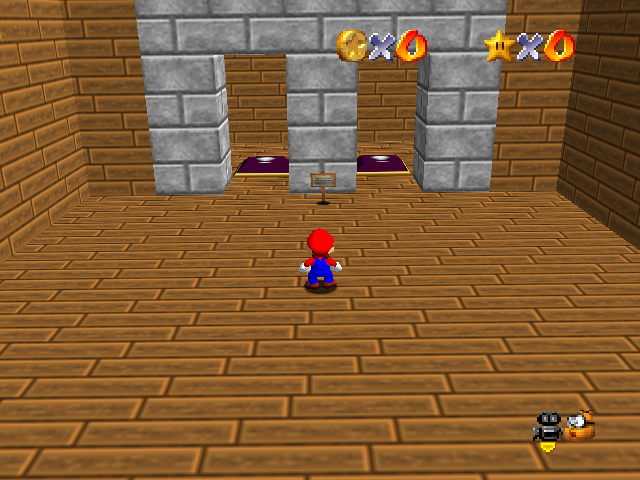
\includegraphics[width=0.8\textwidth]{./Pictures/variable-gadget.png}
    \caption{Gadget de Variable}
    \label{var-gadget}
\end{figure}


Como se puede observar el gadget de cada variable es una habitación con dos salidas. La puerta de la izquierda representa el camino True
y la de la derecha el camino False. Una vez que se cruza una de estas puertas Mario presionará el botón que se encuentra en el umbral
de la puerta lo que activará un mecanismo que le impedirá regreasar y revertir su decisión.

Según el camino que escoja el jugador este le conducirá a los gadgets de las cláusulas en las que ese literal esté presente. Un gadget de
cláusula consiste en una habitación con una moneda roja como se puede observar en la figura~\ref{clause-gadget} . Hay $l$ monedas rojas, una por cada cláusula. El objetivo del jugador es 
coleccionar todas estas para desbloquear la estrella en el Check gadget. Cada vez que el jugador sale de un gadget de variable
el camino que tome le conducirá por los gadgetes de cláusulas en las que ese literal está presente. Una vez que termine de recorrer todas esas
cláusulas el camino le conducirá al gadget de la siguente variable y se repite el proceso nuevamente.

\begin{figure}[htbp]
    \centering
    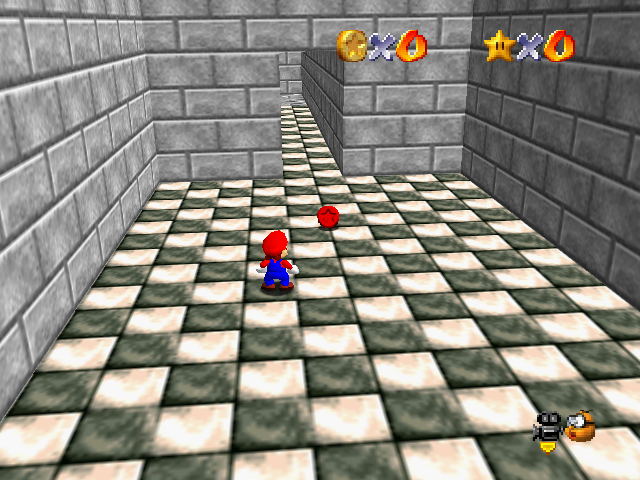
\includegraphics[width=0.8\textwidth]{./Pictures/clausule-gadget.png}
    \caption{Gadget de Cláusula}
    \label{clause-gadget}
\end{figure}

Una vez que ya se recorrieron todas los gadgets de variables o todos los de cláusulas el camino conducirá al jugador al Check gadget~\ref{check-gadget}.
En caso de que Mario haya pasado por todas las cláusulas y coleccionado las monedas rojas entonces la estrella aparecerá y Mario podrá
obtenerla para completar el nivel, en caso de que Mario no haya pasado por todas las cláusulas la estrella no aparecerá.

\begin{figure}
    \centering
    \begin{minipage}{0.45\textwidth}
        \centering
        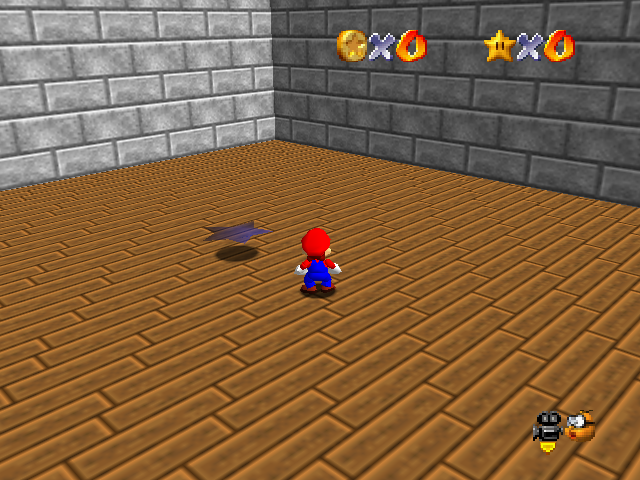
\includegraphics[width=\textwidth]{./Pictures/finish-not-satisfiable.png}
    \end{minipage}
    \hfill
    \begin{minipage}{0.45\textwidth}
        \centering
        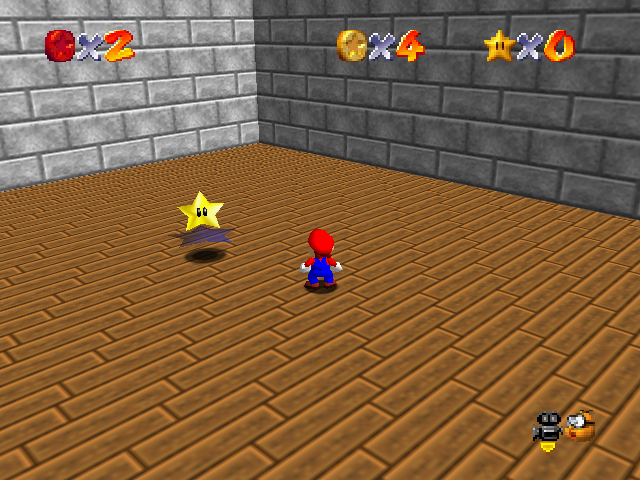
\includegraphics[width=\textwidth]{./Pictures/finish-satisfiable.png}
    \end{minipage}
    \caption{Check gadget}
    \label{check-gadget}
\end{figure}

Nos queda probar que nuestra insctancia de 3-SAT es satisfacible ssi el nivel que creamos es completable.

Supongamos que $S$ es satisfacible y sea $v$ una asignación satisfacible. Si $v(x_i)$ es True Mario debe tomar 
la puerta que conduce por el camino True en el gadget de la variable $x_i$, si $v(x_i)$ es False Mario debe tomar
el camino False. Como $v$ es una asignación satisfacible al menos un literal de cada cláusula toma valor True y de esta
forma aseguramos que Mario obtenga todas las menos rojas disponibles en las cláusulas. Finalmente cuando Mario llegue A
al gadget Check la estrella estará disponible y podrá terminar el nivel.

Por otro lado supongamos que el nivel es completable. Si el nivel es completable existe un camino desde el inicio el cual
pasa por todas las cláusulas y desbloquea la estrella en el Check gadget. Dependiendo de la puerta que escoja Mario en cada gadget de varible podemos construir
una asignación satisfacible para S, si escogió el camino True para la variable $x_i$ entonces le asignamos valor True a $x_i$ y si 
escogió el camino False le asignamos el valor False.

Por tanto podemos afirmar que completar un nivel de Mario 64 generalizado es NP-Hard.

\end{proof}


%
% ---- Bibliography ----
%
% BibTeX users should specify bibliography style 'splncs04'.
% References will then be sorted and formatted in the correct style.
%
% \bibliographystyle{splncs04}
% \bibliography{mybibliography}
%
\begin{thebibliography}{8}


\bibitem{ref_url2}
Mario Wiki, \url{https://www.mariowiki.com/Super_Mario_64} 

\end{thebibliography}
\end{document}
